\documentclass{beamer}
\usecolortheme{dolphin}
%\usetheme{Warsaw}

\usepackage{amsmath,amssymb,amsrefs}
\usepackage{amscd}
\usepackage{latexsym}
\usepackage{graphics}
\usepackage{subfigure}
\usepackage{placeins}
\usepackage{booktabs}
\usepackage{multirow}
\usepackage{times}  % fonts are up to you
\usepackage[authoryear]{natbib}
\def\newblock{\hskip .11em plus .33em minus .07em} %this line is used to
% fix the bug of natbib that ``\newblock'' undefined.
\usepackage{array}

\usepackage{lipsum}

 \setbeamersize{text margin left=11pt,text margin right=8pt}



\newcommand\mydef{\mathrel{\overset{\makebox[0pt]{\mbox{\normalfont\tiny\sffamily def}}}{=}}}

\usepackage{soul}



\newif\ifpaper

% \papertrue % or
\paperfalse


\usepackage{graphicx}
\usepackage{nicefrac}
\usepackage{lscape}
\usepackage{times}
% \usepackage[dvips,colorlinks=true,linkcolor=red,filecolor=green,citecolor=red]{hyperref}
%\usepackage[]{amsmath,amssymb,epsfig}
% \usepackage{subfigure}
\usepackage{mathtools}%
\usepackage{algorithm}
\usepackage{algorithmic}
\usepackage{wrapfig}





\newcommand{\mb}[1]{\mbox{\boldmath$#1$}}

\setbeamertemplate{headline}{\scriptsize{\vspace*{0.1cm}\hspace*{0.1cm}\insertframenumber}}

\title{Discovering Hidden Prerequisites}
\author{ Anumat Srivastava, Lowell Bander, Paul Jayazeri\\
\vspace{5mm}
MATH 191 Topics in Data Science, UCLA}
% \institute[]{ Applied Mathematics, UCLA
% Applied and Computational Mathematics, \\
% Princeton University
% }
%\address{PACM Graduate Student Seminar}
% \date{ Harvard University \\ February 24, 2014}

\date{ \today}

% note: do NOT include a \maketitle line; also note that this title
% material goes BEFORE the \begin{document}

%%%%% have this if you'd like a recurring outline
\AtBeginSection[]  % "Beamer, do the following at the start of every section"
{
\begin{frame}<beamer>
  \frametitle{Outline} % make a frame titled "Outline"
  \tableofcontents[currentsection]  % show TOC and highlight current section
\end{frame}
}


\begin{document}

\newtheorem{theo}{Theorem}
\newtheorem{lem}{Lemma}
\newtheorem{defin}{Definition}
\newtheorem{prop}{Proposition}
\newtheorem{ex}{Example}
\newtheorem{alg}{Algorithm}
\newtheorem{cor}{Corollary}
\newtheorem{case}{Case}


% this prints title, author etc. info from above
\begin{frame}
  \titlepage
\end{frame}



\section{Introduction}

\begin{frame}
     \frametitle{Introduction}
\begin{itemize}
\item The objective is to use ranking algorithms to discover hidden prerequisites in the Math and Computer Science curriculums 
\item  We have access to data containing 13,000+ students' GPA's and the order in which they have taken their classes
\item  We will be using the rank centrality and serial rank algorithms to rank the courses
\item By contrasting the different orderings of classes taken for high gpa students vs. low gpa students, we should be able to find courses that should precede other courses
\end{itemize}
\end{frame}



\section{Our Work}
\subsection{Serial Rank}
\begin{frame}
     \frametitle{Serial Rank}
\begin{itemize}
\item For Serial Rank, we use a matrix C of size n x n of pairwise comparisons (where n is the number of courses offered by the CS/Math departments), defined as follows :
\begin{equation}
C_{ij} = \left\{
	\begin{array}{rl}
 1 & \text{ if course i is taken before course j (or i=j)} 	\\
 &  \\
 0 & \text{ for i and j are tied or have no available comparison }	\\
 &  \\
 -1 & \text{ if course j is taken before course i} 
     \end{array}
   \right.
\label{myExpValue}
\end{equation}
The pairwise similarity matrix is constructed as follows

$$S_{ij}^{match} = \sum_{k=1}^{n}(\frac{1+C_{ik}C_{jk}}{2})$$
Then compute the Laplacian matrix $L_{S} = diag(S1) - S$ and finally computing and sorting the Fiedler vector of S will give the ranking. 

\end{itemize}
\end{frame} 

\begin{frame}
     \frametitle{Serial Rank}
\begin{itemize}
\item For Serial Rank, we shall split the data into sets of high gpa students and low gpa students.
\item Then we build similarity matrices for each student in both sets as described in the previous slide
\item We combine all the similarity matrices into 1 normalized similarity matrix for each set and look at the pairwise difference of each entry in the two matrices.
\item If the difference is large, the course taken by the high gpa students should be a prerequisite to the course taken by the low gpa students!
\item We then use these two similarity matrixes to rank courses according to the algorithm described.
\end{itemize}
\end{frame}

\subsection{Rank Centrality}
\begin{frame}
     \frametitle{Rank Centrality}
\end{frame}

\section{Summary and conclusion}  \label{sec:conclusion}

\begin{frame}
\frametitle{Summary of our work}
\begin{itemize}
%\item We hope to discover some hidden prerequisites in the curriculums and improve the experience for future UCLA students by presenting our findings to the respective departments
%\item We hope to arrive at prerequisites empirically, 
\item Currently, prerequisites are rather static, at times arbitrary, and thus sometimes inaccurate 
\begin{itemize}
\item Some courses are prerequisites for others when they need not be
\item Some courses ought to be taken before others, but are not presently listed as prerequisites
\end{itemize}
\item We hope to empirically validate whether courses should be prerequisites
\item From this we can generate a directed acyclic graph which optimizes total understanding of Math/Computer Science
\end{itemize} 
\centerline{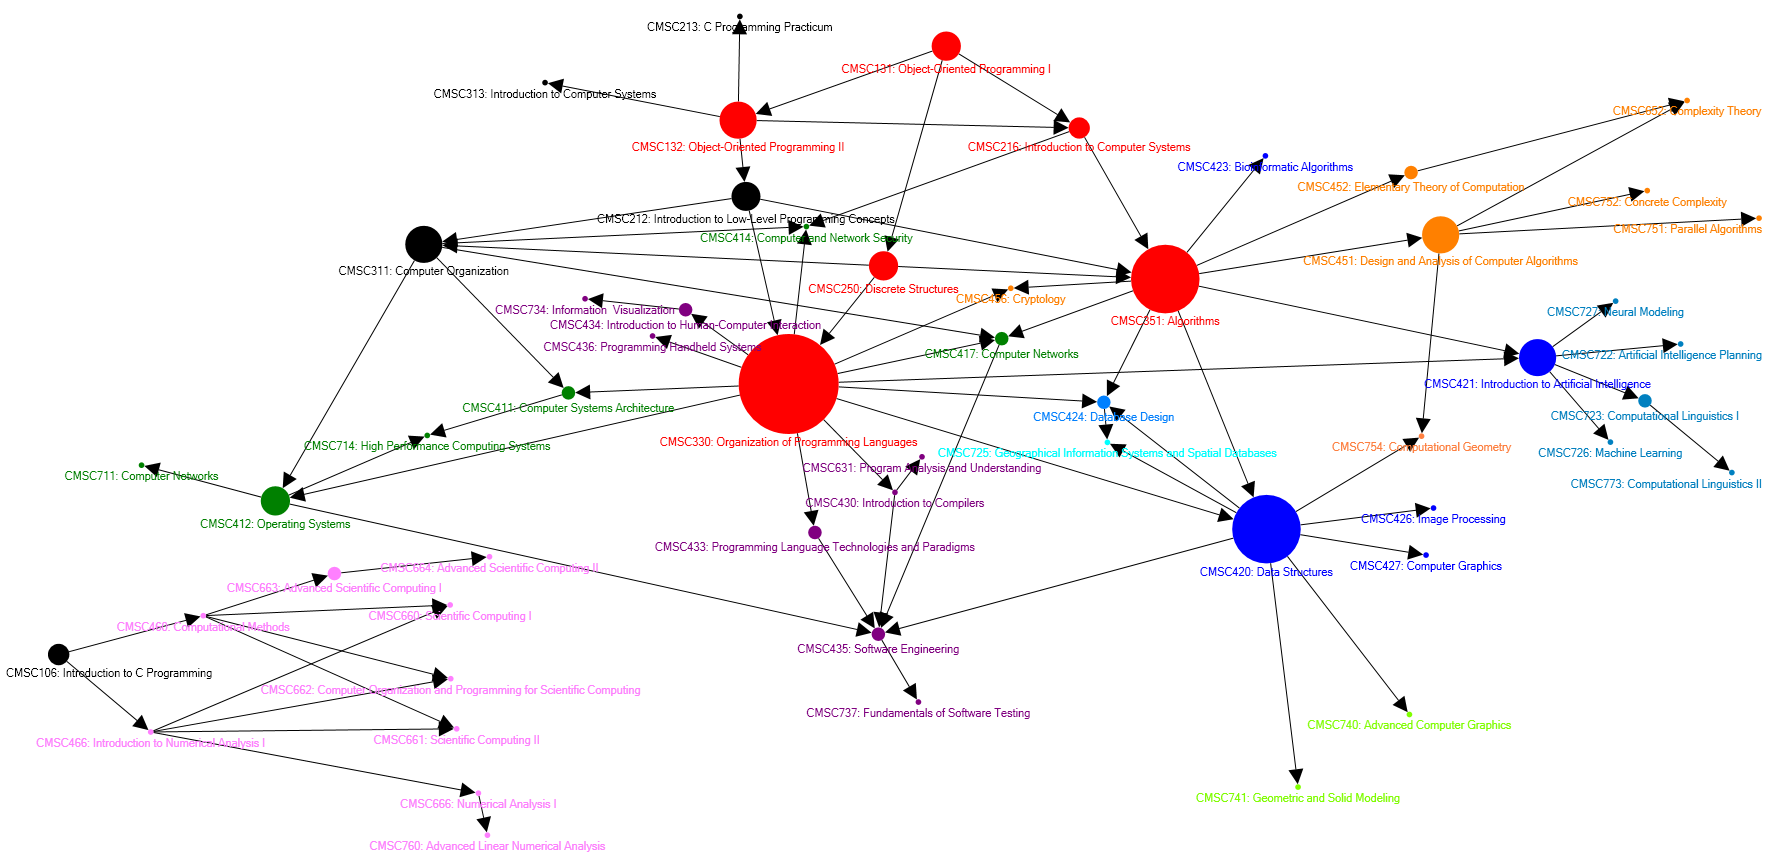
\includegraphics[width=0.76\columnwidth]{dag.png}}
\end{frame}
\end{document}




